\documentclass[11pt,a4paper,fleqn]{article}
\usepackage[utf8]{inputenc}
\usepackage{bsymb}
%usepackage[space]{ctex}
\usepackage{natbib}
\usepackage{graphicx}
\usepackage{algorithmic_pf}
\usepackage{indentfirst}
\usepackage[export]{adjustbox}
\usepackage{etoolbox}
\expandafter\patchcmd\csname Gin@ii\endcsname
  {\setkeys {Gin}{#1}}
  {%
    \setkeys {Gin}
      {max width=\textwidth,max height=.5\textwidth,keepaspectratio,#1}%
  }
  {}{}
\title{Homework 4,5}

\author{10175101126,10175101226,10175101117}
\date{April 2019}
\setkeys{Gin}{max width=\linewidth}
\begin{document}
\maketitle

\section{ homework 2.4 }
\subsection{Rewrite PRE and POST }
\noindent
Add the prove process here: \\
%\setlength{\hangindent}{2em}



\subsection{Prove the invariants}
\noindent


\subsection{ Prove POST}
\noindent




\subsection{Propose a variant and prove it}
\noindent


\subsection{Translate this program to C and execute it}
\noindent
Program is listed here:\\
\begin{figure}[h!]
\centering
\includegraphics{}
\caption{ write in c}
\label{fig}
\end{figure}


\section{homework 2.5}

\subsection{Exercise 1: terminate this proof}
\noindent
case1:\\
$m \in (k + 1)+1 \upto j$\\
$\forall m \cdot m \in k+1 \upto j \Rightarrow g(m) > x  $\\
$\forall m \cdot m \in 0 \upto k \Rightarrow g(m) \leq x $\\
$g(j+1) \leq x $\\
$\vdash$\\
$h(m)>x $\\

\noindent
where h is $ (\{k+1, j+1\} \domsub g) \cup\{k+1 \mapsto g(j+1), j+1 \mapsto g(k+1)\}$\\
\noindent so we have:\\
$h(m) = g(m)$ since $m>k+1 $ and $m<j+1$\\ 
\noindent Applying rule \text{U}\_\text{H}:\\
$g(m)>x $\\
$ \forall m \cdot m \in 0 \upto k \Rightarrow g(m) \leq x $\\
$g(j+1) \leq x $\\
$m \in (k + 1)+1 \upto j$\\
$\vdash$\\
$g(m)>x \quad \text{HYP}$\\

\noindent
case2($m = j+1 $):\\



\subsection{Exercise 2: terminate this proof}
\noindent




\subsection{Exercise 3}

\subsubsection{Rewrite PRE- and POST-conditions}


\subsubsection{Prove all invariants}

\subsubsection{Prove POST}
\noindent
$ \text{PRE},$
$j=n-1,$
$j\in -1\upto n-1,$
$k\in -1\upto j,$\\
$g\in 0\upto n-1\rightarrowtail\mathbb{N},$
$ran(g)=ran(f),$\\
$ \forall m \cdot m \in 0 \upto k \Rightarrow g(m) \leq x ,$\\
$ \forall m \cdot m \in k+1 \upto j \Rightarrow g(m)>x$\\
$\vdash$\\
$k\in -1\upto n-1,$
$g\in 0\upto n-1\rightarrowtail\mathbb{N},$
$ran(g)=ran(f),$\\
$ \forall m \cdot m \in 0 \upto k \Rightarrow g(m) \leq x ,$\\
$ \forall m \cdot m \in k+1 \upto n-1 \Rightarrow g(m)>x$\\
\\
$\text{PRE},$
$n-1\in -1\upto n-1,$
$k\in -1\upto n-1,$\\
$g\in 0\upto n-1\rightarrowtail\mathbb{N},$
$ran(g)=ran(f),$\\
$ \forall m \cdot m \in 0 \upto k \Rightarrow g(m) \leq x ,$\\
$ \forall m \cdot m \in k+1 \upto n-1 \Rightarrow g(m)>x$\\
$\vdash$\\
$k\in -1\upto n-1,$
$g\in 0\upto n-1\rightarrowtail\mathbb{N},$
$ran(g)=ran(f),$\\
$ \forall m \cdot m \in 0 \upto k \Rightarrow g(m) \leq x ,$\\
$ \forall m \cdot m \in k+1 \upto n-1 \Rightarrow g(m)>x\quad \text{HYP\quad and\quad EQL}$\\



\subsubsection{Propose a variant and prove it}
\noindent
since j increases all the time, we choose n-1-j as the variant.\\ 
\\
$\text{NAT:}$\\
$ \ldots,j\in -1\upto n-1\vdash n-1-j\in \mathbb{N}$\quad since $j\leq n-1$\\
$\text{VAR:}$\\
$ \ldots,g(j+1)>x\vdash[j:=j+1]n-1-j<n-1-j$\\
$ \ldots,g(j+1)>x\vdash n-1-(j+1)<n-1-j$\\
$ \ldots,g(j+1)>x\vdash -1<0$\\
Obvious since $-1<0$\\
$ \ldots,g(j+1)\leq x\vdash[j:=j+1;g:=h;k:=k+1]n-1-j<n-1-j$\\
$ \ldots,g(j+1)\leq x\vdash[j:=j+1][g:=h][k:=k+1]n-1-j<n-1-j$\\
$ \ldots,g(j+1)\leq x\vdash[j:=j+1][g:=h]n-1-j<n-1-j$\\
$ \ldots,g(j+1)\leq x\vdash[j:=j+1]n-1-j<n-1-j$\\
$ \ldots,g(j+1)\leq x\vdash n-1-j-1<n-1-j$\\
$ \ldots,g(j+1)\leq x\vdash -1<0$\\
Obvious since $-1<0$\\

\subsubsection{Translate the program to C and run it}
Program is listed here:\\

\begin{figure}[h!]
\centering
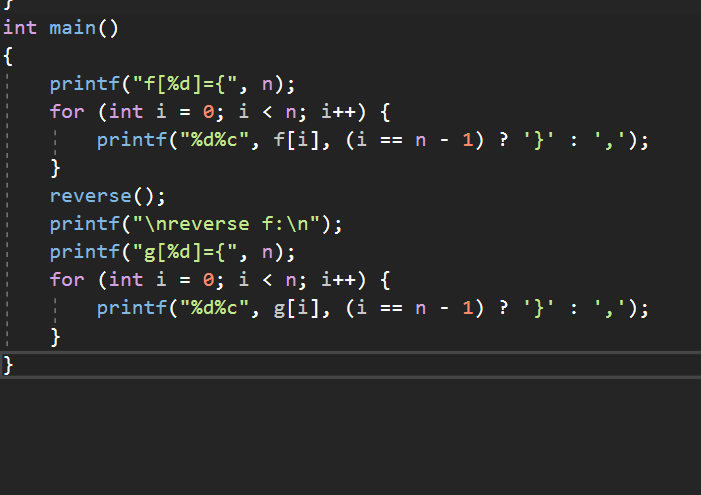
\includegraphics{2.png}
\caption{ write in c}
\label{fig}
\end{figure}

\begin{figure}[h!]
\centering
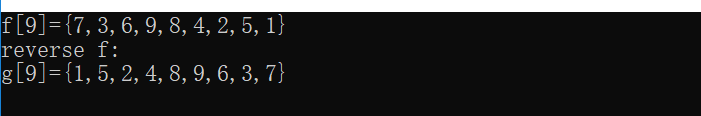
\includegraphics{3.png}
\caption{ write in c}
\label{fig}
\end{figure}

\begin{figure}[h!]
\centering
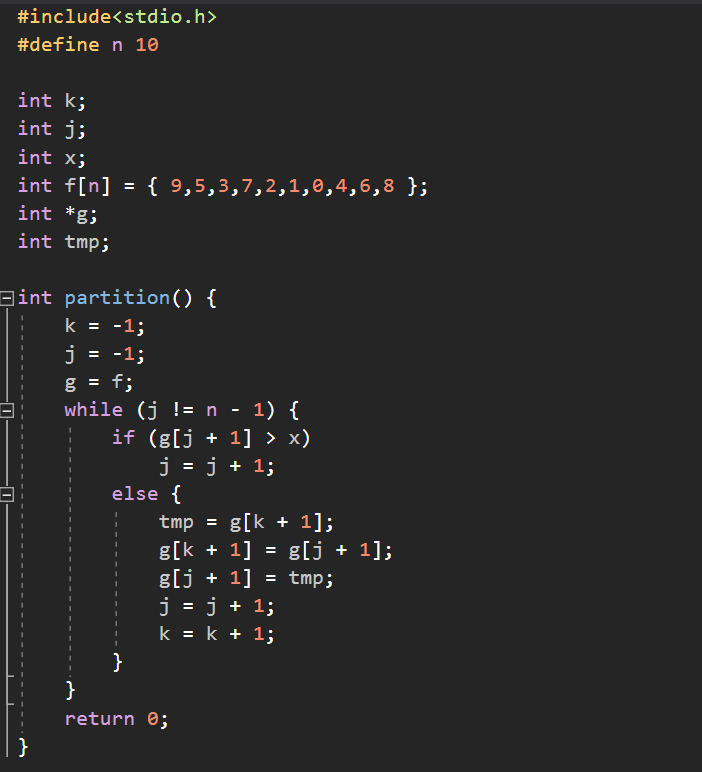
\includegraphics{4.png}
\caption{ run }
\label{fig}
\end{figure}



%\bibliographystyle{plain}
%\bibliography{references}
\end{document}
